\subsection{Загрузка файлов}
В данном разделе будет показано, как устанавливать программу и пользоваться ей. Для описания каждого проделанного шага будут включены описание действий и скриншоты приложения.
\subsubsection{Установка программы}
Дистрибутив данной программы можно будет получить по ссылке, считав ее с
прилагаемого qr-кода(рис. \ref{ref})

\begin{figure}[h!]
    \centering
    
\includegraphics[width=0.7\textwidth]{./screenshots/qr-code.png}
    \caption{ссылка на программу}
    \label{ref}
\end{figure}

Чтобы начать испытания выполнения требований к функциональным характеристикам,
необходимо запустить установщик программы путем нажатия на его иконку. После
запуска установщика появится приветственное окно мастера установки (рис. \ref{install}).

\begin{figure}[h!]
    \centering
    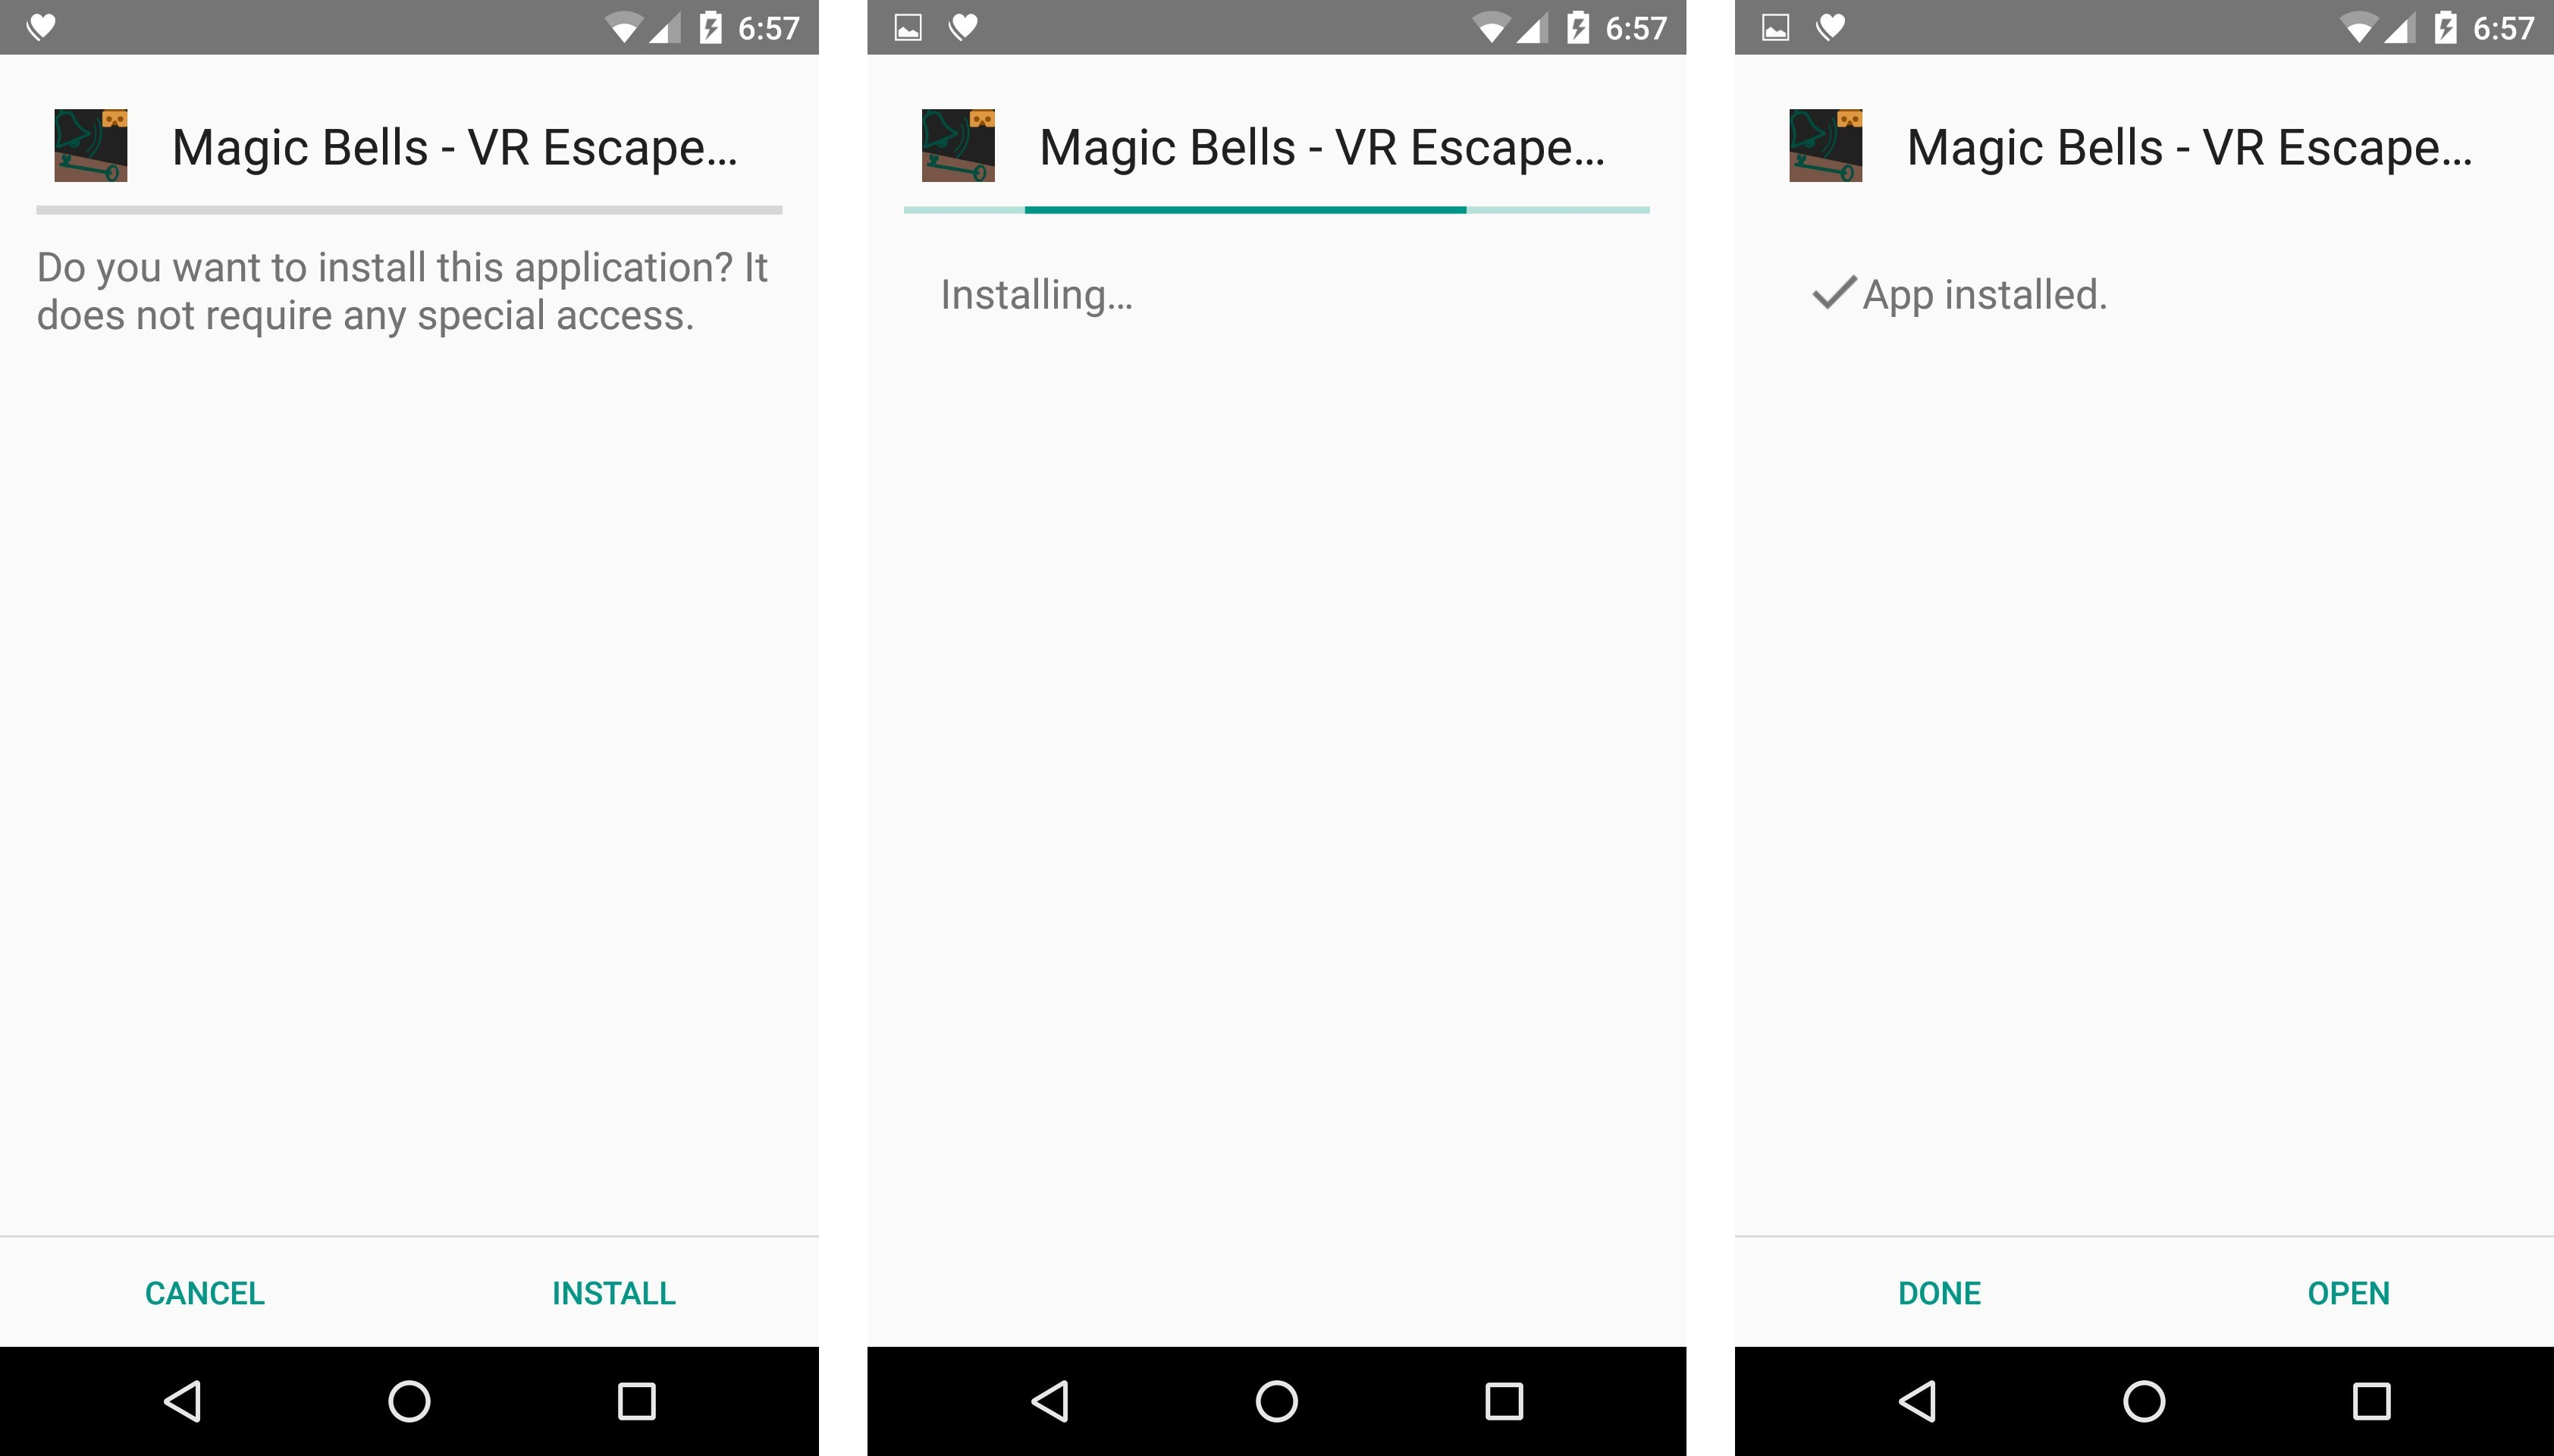
\includegraphics[width=0.9\textwidth]{./screenshots/install.jpg}
    \caption{процесс установки программы}
    \label{install}
\end{figure}

\subsubsection{Процесс игры}
Затем приложение необходимо открыть. Оператора будет приветствовать экран выбора режима игры. Это либо VR Mode, либо Normal Mode (рис. \ref{modes}).
\begin{figure}[h!]
    \centering
    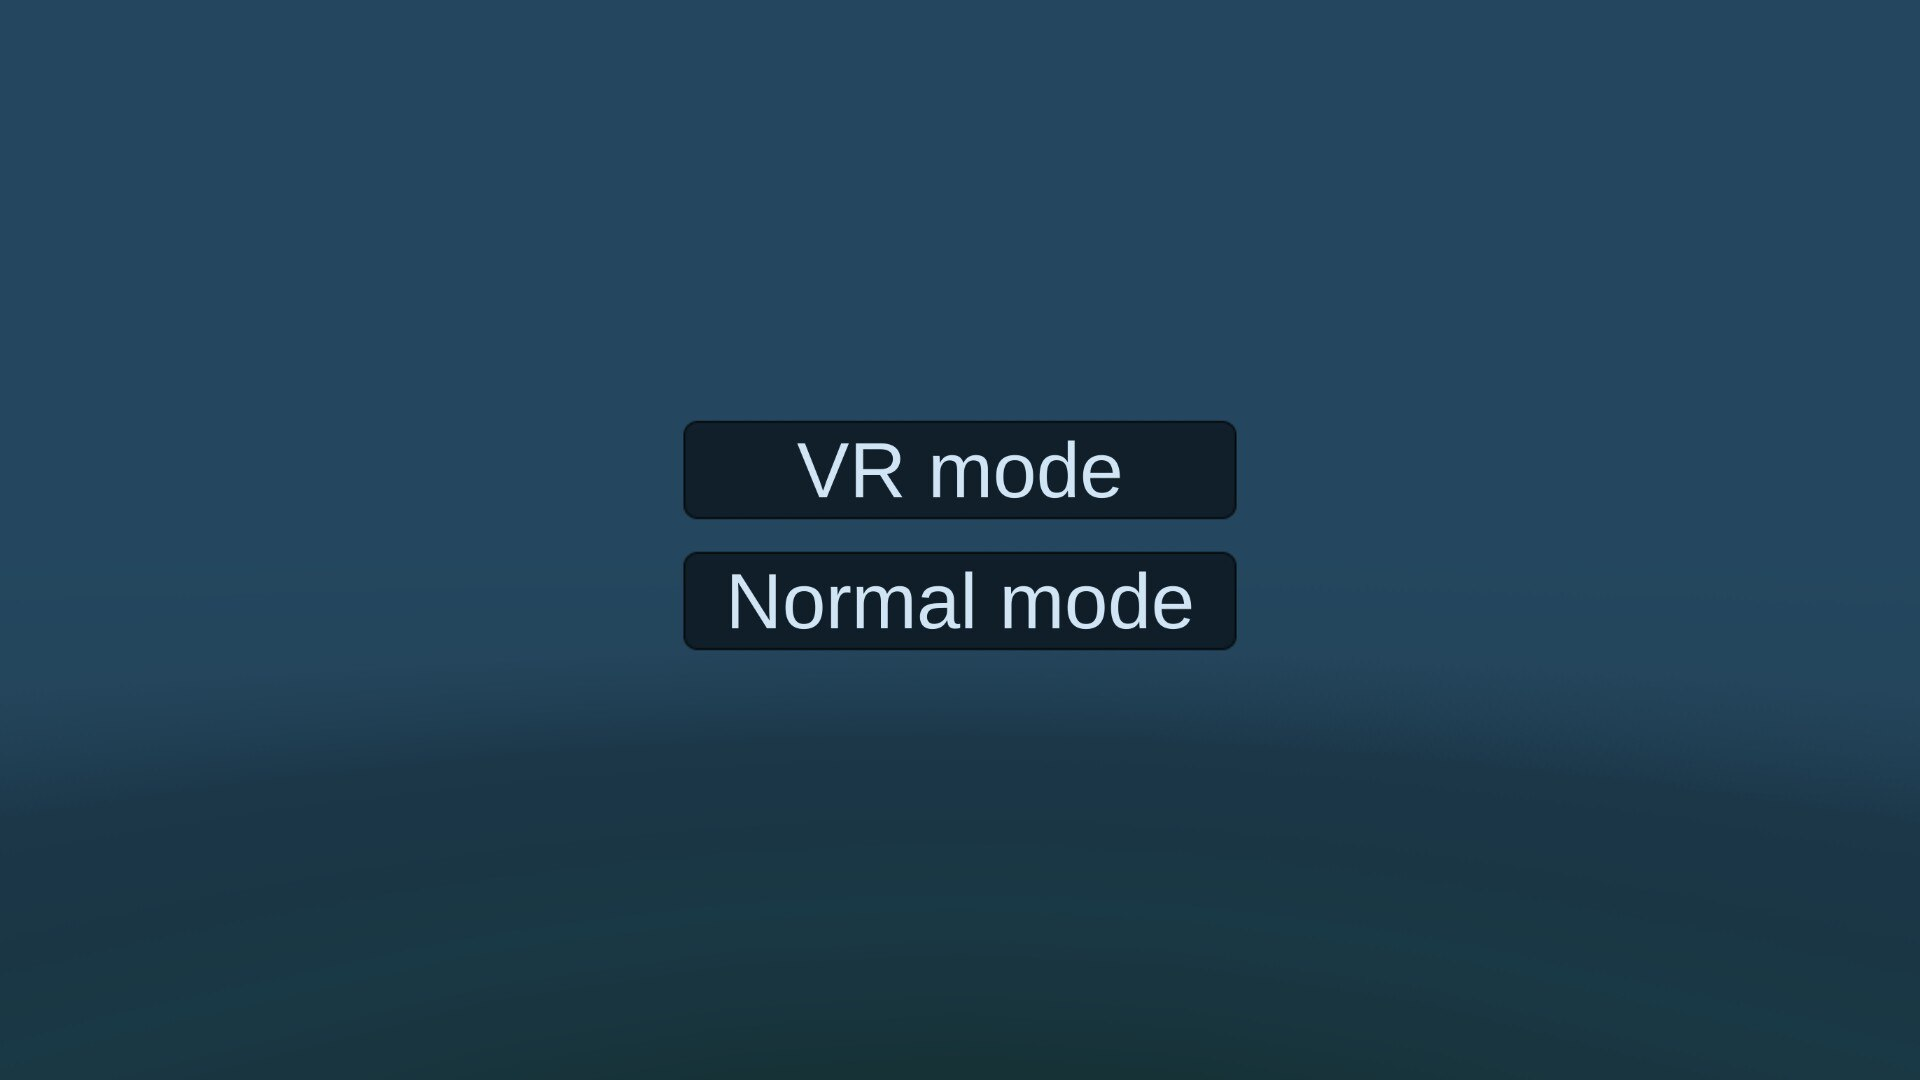
\includegraphics[width=0.8\textwidth]{./screenshots/modes.jpg}
    \caption{\small{меню переключения режима}}
    \label{modes}
\end{figure}

Выбрав режим, можно начать игру. Цель игры - выбраться из запертого помещения при помощи ключа. Ключ надо найти, решив цепочку головоломок. 

Оператору будут показываться вспомогательные сообщения, сообщающие сюжет и цель игры. Будет проведена тренировка, в которой предложится поднять и бросить камень с дороги. 
\begin{figure}[h!]
    \centering
    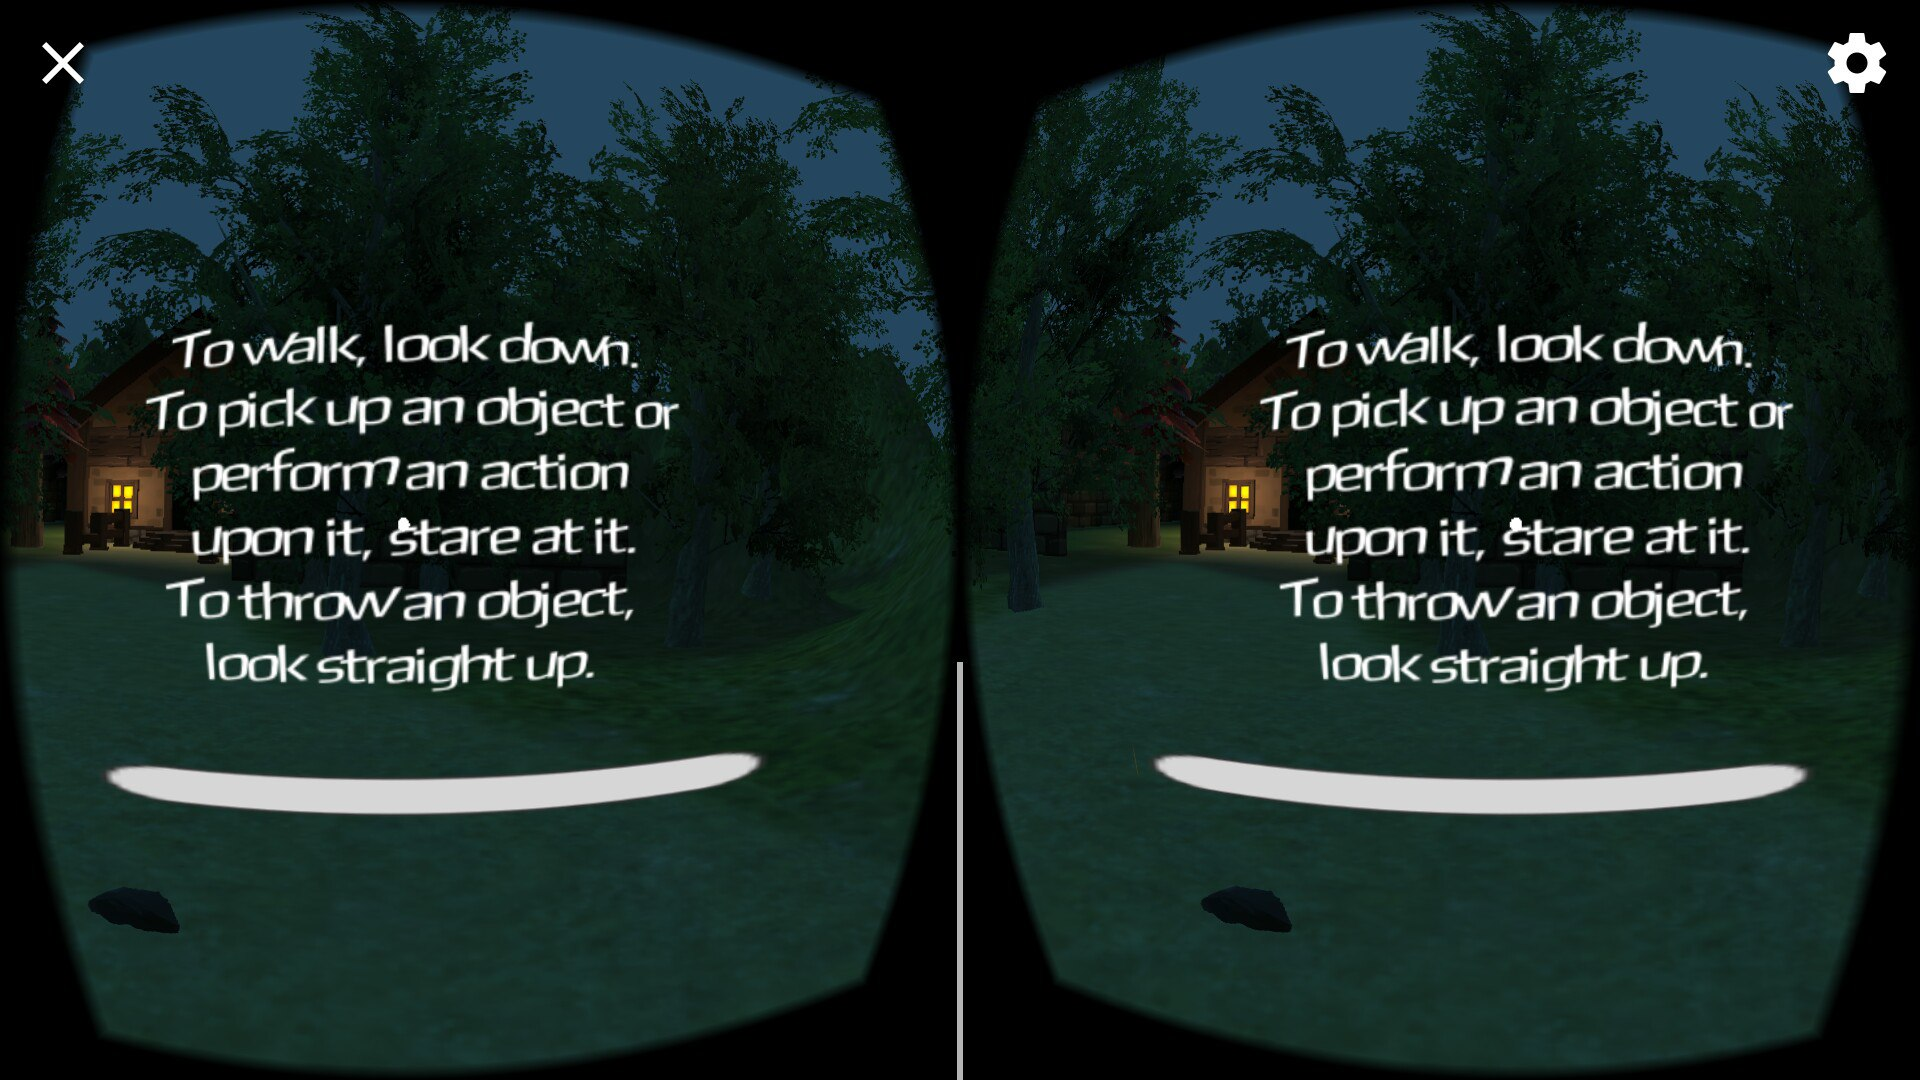
\includegraphics[width=0.8\textwidth]{./screenshots/tutorial.jpg}
    \caption{\small{объяснение правил управления в игре}}
    \label{tutorial}
\end{figure} 

\begin{figure}[h!]
    \centering
    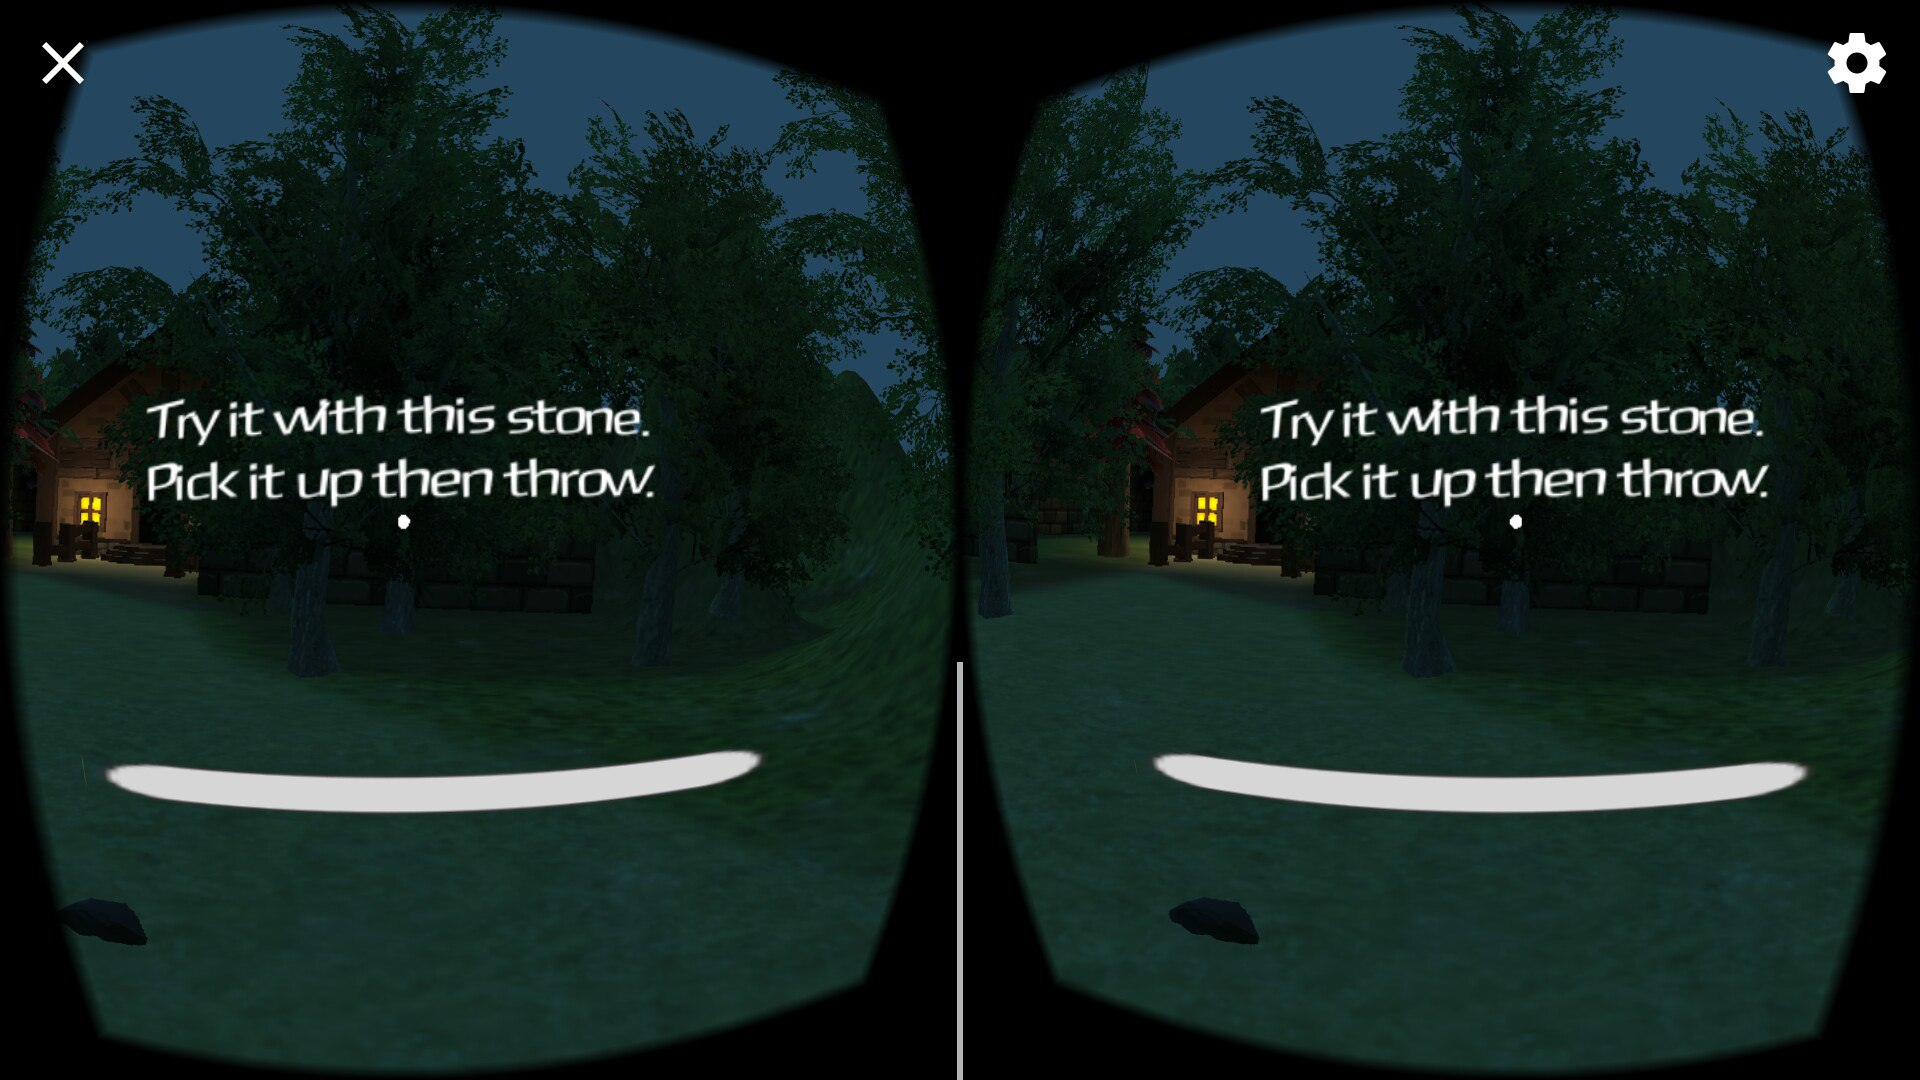
\includegraphics[width=0.8\textwidth]{./screenshots/try.jpg}
    \caption{\small{приглашение к тренировке}}
    \label{try}
\end{figure} 

\begin{figure}[h!]
    \centering
    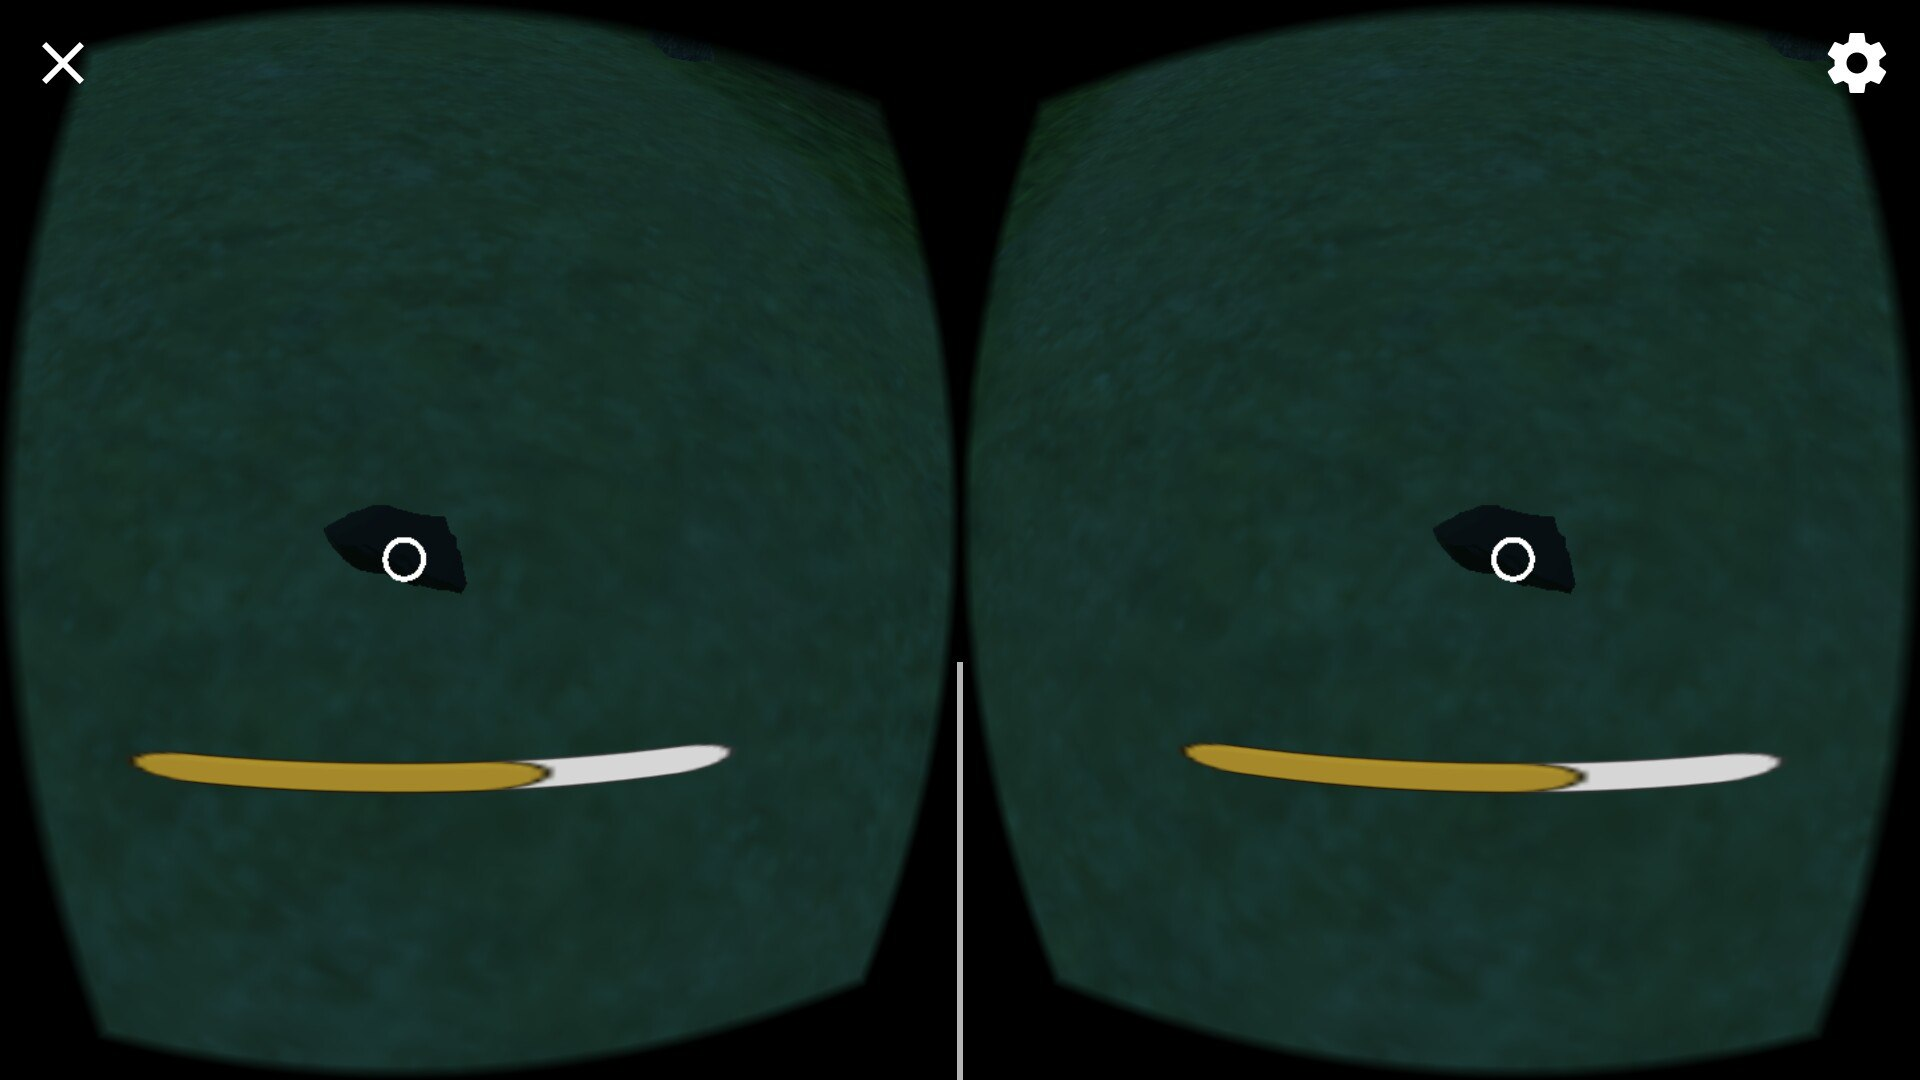
\includegraphics[width=0.8\textwidth]{./screenshots/pick_stone1.jpg}
    \caption{\small{ожидание выполнения действия над объектом камень}}
    \label{pick_stone}
\end{figure} 

\begin{figure}[h!]
    \centering
    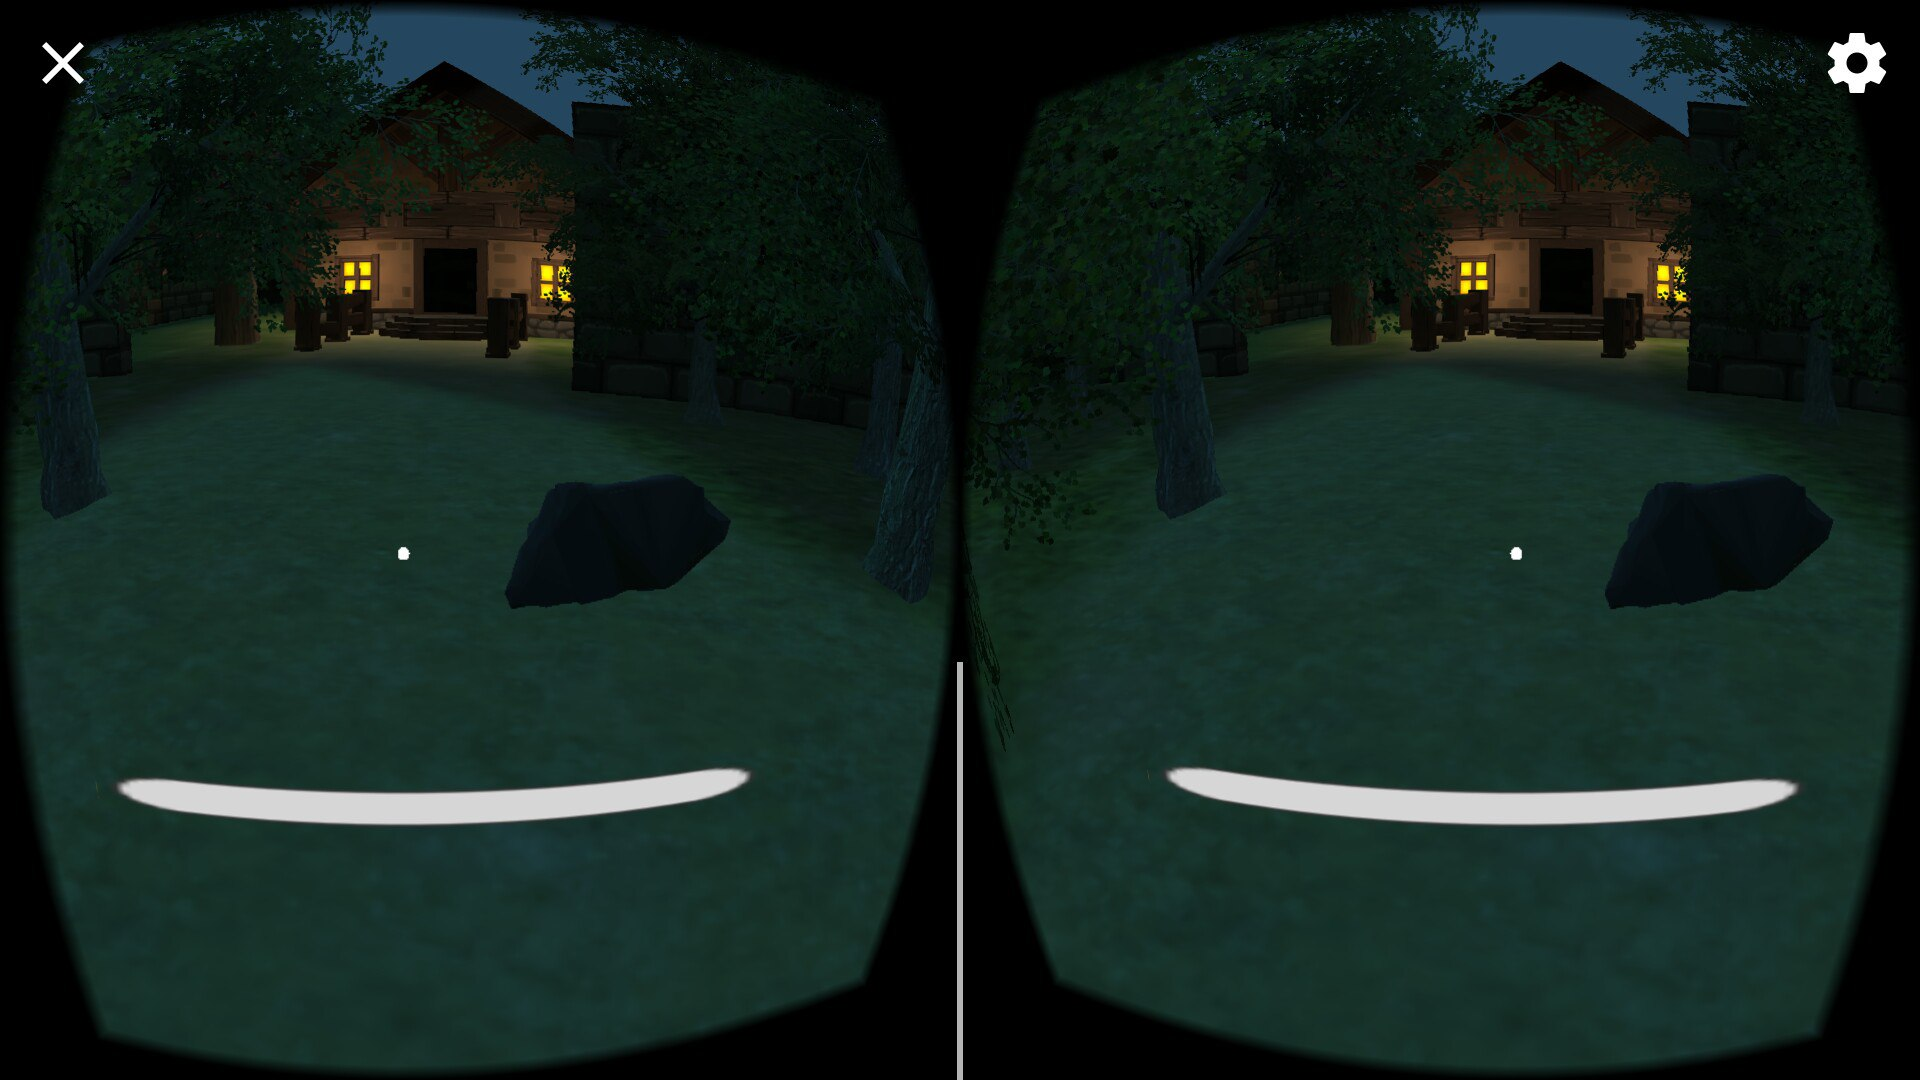
\includegraphics[width=0.8\textwidth]{./screenshots/picked_stone1.jpg}
    \caption{\small{результат выполнения действия над объектом - камень в руке}}
    \label{picked_stone}
\end{figure} 
\newpage
Далее взаимодействие со всеми игровыми объектами происходит аналогичным образом.
После, игрок попадает в дом, в основное место действия. При помощи наводок, таких как записка на столе и подсветка картины после решения головоломки с колокольчиками, игрок сможет дойти до конца, найти ключ и выбраться из заперти.

\newpage

